Taking magnitudes in \(z^4=1\) gives \(\lvert z\rvert=1\). Since every solution lies on the unit circle, it can be written as \(z=e^{i\theta}\), which gives

\[
e^{i4\theta}=1=e^{i2\pi k},\qquad k\in\mathrm{Z}.
\]

Equating the exponents yields \(4\theta=2\pi k\), so \(\theta=k\pi/2\). Since increasing \(k\) by four adds one full revolution, four consecutive values of \(k\) give all distinct roots.

\[
\boxed{z\in\{1,\ i,\ -1,\ -i\}}
\qquad\text{(C.9.1.a)}
\]

Using \(k=0,1,2,3\), the same roots in complex-exponential form are

\[
\boxed{z_k=e^{ik\pi/2},\qquad k=0,1,2,3}
\qquad\text{(C.9.1.b)}
\]

Euler's identity combines the real and imaginary parts of a unit-magnitude complex exponential. Therefore, substituting \(\alpha=\omega t\) gives

\[
\boxed{e^{i\omega t}=\cos(\omega t)+i\sin(\omega t)}
\qquad\text{(C.9.2)}
\]

Writing each sinusoid as \(x(t)=\sin(\omega t+\phi)\) identifies \(\phi\) as its phase. I define the phase difference as the phase of the second signal minus the phase of the first,

\[
\Delta\phi=\phi_2-\phi_1.
\]

With this definition, a positive value means that \(x_2(t)\) leads \(x_1(t)\). For part (a), \(\phi_1=0\) and \(\phi_2=3\pi/4\), so

\[
\boxed{\Delta\phi_a=\frac{3\pi}{4}=135^\circ}
\qquad\text{(C.9.3.a)}
\]

For part (b), subtracting the first phase from the second and using a common denominator gives

\[
\Delta\phi_b=\frac{3\pi}{4}-\frac{\pi}{3}
=\frac{9\pi-4\pi}{12}=\frac{5\pi}{12}.
\]

Therefore,

\[
\boxed{\Delta\phi_b=\frac{5\pi}{12}=75^\circ}
\qquad\text{(C.9.3.b)}
\]

For part (c), subtracting the phases in degrees and then converting the result to radians gives

\[
\Delta\phi_c=115^\circ-45^\circ=70^\circ
=70\left(\frac{\pi}{180}\right)=\frac{7\pi}{18}.
\]

\[
\boxed{\Delta\phi_c=\frac{7\pi}{18}=70^\circ}
\qquad\text{(C.9.3.c)}
\]

The phase of \(e^{i\theta}\) is \(\theta\) modulo \(2\pi\). When an angle has more than one equivalent representation, I use the principal phase interval \((-\pi,\pi]\). Therefore, the requested phases are

\[
\boxed{\arg\left(e^{i\pi/2}\right)=\frac{\pi}{2}=90^\circ}
\qquad\text{(C.9.4.a)}
\]

For \(e^{i3\pi/2}\), the given angle is \(270^\circ\). Subtracting \(360^\circ\) gives the equivalent principal phase \(-90^\circ\),

\[
\boxed{\operatorname{Arg}\left(e^{i3\pi/2}\right)=-\frac{\pi}{2}=-90^\circ,
\qquad \frac{3\pi}{2}\equiv-\frac{\pi}{2}\pmod{2\pi}}
\qquad\text{(C.9.4.b)}
\]

\[
\boxed{\arg\left(e^{i\pi/4}\right)=\frac{\pi}{4}=45^\circ}
\qquad\text{(C.9.4.c)}
\]

\[
\boxed{\arg\left(e^{-i\pi/2}\right)=-\frac{\pi}{2}=-90^\circ}
\qquad\text{(C.9.4.d)}
\]

\[
\boxed{\arg\left(e^{-i\pi/4}\right)=-\frac{\pi}{4}=-45^\circ}
\qquad\text{(C.9.4.e)}
\]

For item (5), the unit-circle coordinates are \(\bigl(\cos\theta,\sin\theta\bigr)\). Therefore, \(e^{i\pi/2}\) lies at \((0,1)\), \(e^{i3\pi/2}\) at \((0,-1)\), \(e^{i\pi/4}\) at \((\sqrt{2}/2,\sqrt{2}/2)\), and \(e^{-i\pi/4}\) at \((\sqrt{2}/2,-\sqrt{2}/2)\). Since the angles \(3\pi/2\) and \(-\pi/2\) differ by one full revolution, \(e^{-i\pi/2}\) also lies at \((0,-1)\). Thus, the two expressions represent the same point,

\[
e^{i3\pi/2}=e^{-i\pi/2}=-i.
\]

\begin{figure}[H]
\centering
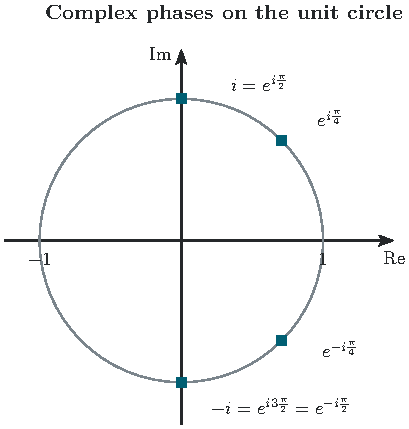
\includegraphics[width=0.7\linewidth,height=0.34\textheight,keepaspectratio,alt={C.9. The requested complex numbers on the unit circle.}]{figures/generated/solutions/C9.pdf}
\caption{C.9.5. Requested points on the unit circle.}
\end{figure}

\[
\boxed{e^{i3\pi/2}=e^{-i\pi/2}=-i}
\qquad\text{(C.9.5)}
\]

For item (6), the real and imaginary parts of \(Z=4+5i\) are \(4\) and \(5\), respectively. Therefore, the magnitude is

\[
\lvert Z\rvert=\sqrt{4^2+5^2}=\sqrt{41}=6.4031.
\]

Since \(Z\) lies in the first quadrant, the ordinary inverse tangent of the imaginary part divided by the real part gives its phase,

\[
\arg Z=\tan^{-1}\left(\frac{5}{4}\right)=0.8961\ \mathrm{rad}
=51.3402^\circ.
\]

\[
\boxed{\lvert Z\rvert=\sqrt{41}=6.4031,\qquad
\arg Z=0.8961\ \mathrm{rad}=51.3402^\circ}
\qquad\text{(C.9.6)}
\]
